% Executive companion to main.tex. No new experiments or regenerated results.
% Quantitative sources: main.tex and NUMBERS.md in this directory.
% Build from this directory: tectonic main-short-astra.tex
\documentclass[11pt,letterpaper]{article}
\usepackage[margin=0.8in,headheight=15pt]{geometry}
\usepackage[T1]{fontenc}
\usepackage{lmodern}
\usepackage{microtype}
\usepackage{graphicx}
\usepackage{booktabs,tabularx,array}
\usepackage{xcolor}
\usepackage{enumitem}
\usepackage{titlesec}
\usepackage{fancyhdr}
\usepackage{caption}
\usepackage[colorlinks=true,urlcolor=blue!45!black,linkcolor=blue!45!black]{hyperref}
\definecolor{ink}{RGB}{24,53,70}
\definecolor{pale}{RGB}{237,243,246}
\titleformat{\section}{\Large\bfseries\color{ink}}{\thesection}{0.65em}{}
\titleformat{\subsection}{\normalsize\bfseries\color{ink}}{}{0em}{}
\titlespacing*{\section}{0pt}{0pt}{12pt}
\titlespacing*{\subsection}{0pt}{12pt}{4pt}
\setlength{\parindent}{0pt}
\setlength{\parskip}{7pt}
\setlist[enumerate]{leftmargin=1.5em,itemsep=5pt,topsep=3pt,parsep=0pt}
\captionsetup{font=small,labelfont=bf,skip=6pt}
\pagestyle{fancy}
\fancyhf{}
\fancyhead[L]{\small\color{ink}CHILL ZEN}
\fancyhead[R]{\small Executive summary}
\fancyfoot[C]{\small\thepage}
\renewcommand{\headrulewidth}{0.3pt}
\raggedbottom
\newcommand{\takeaway}[1]{\par\medskip\noindent\colorbox{pale}{\parbox{\dimexpr\linewidth-2\fboxsep\relax}{\vspace{5pt}\textbf{#1}\vspace{5pt}}}\par\medskip}
\hypersetup{pdftitle={CHILL ZEN: Generative In-Memory Computing with Fewer Sampling Operations},pdfauthor={M. Alexander Nugent},pdfsubject={Executive summary of the CHILL ZEN technical paper}}
\begin{document}
\thispagestyle{plain}
{\small\bfseries\color{ink}RESEARCH OVERVIEW\enspace /\enspace EXECUTIVE SUMMARY\par}
\vspace{9pt}
{\LARGE\bfseries\color{ink}\raggedright CHILL ZEN: Generative In-Memory Computing\\with Fewer Sampling Operations\par}
\vspace{9pt}
{\large M. Alexander Nugent\par}
Knowm Inc.\hfill September 7, 2026
\vspace{5pt}

\takeaway{CHILL ZEN generates small images in an emulator using about 3,600 noisy lane reads. Its proposed hardware has a nominal energy estimate of 2.0 nanojoules per image, about one eighth of the published eight-step DTM estimate. A complete CHILL ZEN machine has not been built.}

\section{The main idea}
Generative computing must make many choices to produce a new example: which shape to draw, which details to add, and how to make those details agree. Probabilistic hardware aims to make these choices efficiently by using electrical noise as a source of randomness. Its energy cost depends on both the cost of a choice and the number of choices required.

CHILL ZEN reduces the sampling work through a structured representation and a short, fixed generation procedure. It first draws a compact code describing the whole image, adds local detail, and reconciles the two. It does not wait for a repeatedly updated network to settle into an equilibrium sampling distribution. In the demonstrated configuration, generation takes 131 sequential steps, with many lane reads performed in parallel.

A \emph{lane} is a memory circuit that combines selected stored weights into a score. In the proposed hardware, memristors store these weights as electrical conductance. Groups of lanes compete to choose a code symbol. Adding controlled noise makes their choices variable; reducing noise makes repair decisions more consistent. The name, Comparator-Heated In-memory Lane Learning with Zero-Ended Noise, describes this alternation between noisy generation and cold repair.

\subsection{What the study reports}
On binarized Fashion-MNIST, a benchmark of small clothing images, the two-level model achieves Fr\'echet Inception Distance (FID) 18.09 after grayscale training, or 9.69 after direct binary training. Lower FID indicates a closer match to the reference distribution in the chosen image features. The published eight-step Denoising Thermodynamic Model (DTM) reports 24.90. This comparison uses a verified replication scoring pipeline for CHILL ZEN, but retains differences in training splits and uncertainty about the original DTM scoring procedure.

The opportunity is an architecture that spends fewer sampling operations per output. The evidence is a benchmark demonstration in an emulator, coupled to a conditional hardware energy model. The study does not establish performance on large images, language, or production workloads. This companion condenses the existing technical paper; it adds no experiments.

\newpage
\section{How the system makes an image}
The model represents an image as a sum of reusable components. A global \emph{backbone} captures structure across the entire canvas. Small residual patches add what the backbone leaves out. The full representation uses 904 bits plus a supplied class label. Decoding simply adds the selected components; it does not require a learned deep neural decoder.

Each level has separate banks for generation and repair. Generator banks learn to retain multiple supported possibilities. Repair banks learn to correct corrupted combinations. Both use local feedback instructions on the lane weights. Codebooks are fitted separately on the host computer, so local bank learning does not mean that the whole training pipeline runs in memory.

\subsection{One generation, from label to pixels}
\begin{enumerate}
\item \textbf{Specify the class.} Hold a label such as ``shirt'' or ``boot'' throughout generation. The reported headline comparisons supply the label and generate equal numbers from each class.
\item \textbf{Draw the global code.} Choose 128 symbols in sequence, each from 16 candidate lanes. Every choice depends on the label and the symbols already chosen. Controlled noise introduces variation.
\item \textbf{Repair the backbone.} Apply one parallel, low-noise sweep to improve consistency among the global symbols.
\item \textbf{Add local detail.} Draw residual codes for all 49 patch locations in parallel, conditioned on the global code.
\item \textbf{Reconcile and decode.} Apply one joint, low-noise sweep that can change both global and patch symbols. Add the selected components to produce the image.
\end{enumerate}
The 128 sequential choices and three parallel sweeps make 131 generation steps. A proposed in-memory decoder adds one parallel read. The emulator currently performs decoding and rendering in host floating point.

\subsection{Why controlled noise matters}
Combining many memory elements on a lane suppresses their individual noise. At the assumed read voltage, this leaves too little randomness for good generation. A \emph{comparator}, the circuit that helps decide which lane wins, must supply most of it. Thus the design requires a controllable noise source in the readout circuit; device variability alone is insufficient.

In the emulator, hot reads use a 10 millivolt read voltage. The best grayscale FID uses 1 millivolt of comparator noise, while the best binary FID uses 3 millivolts. The grayscale classifier score favors a different setting, 2 millivolts. These are selected points on tested grids, not one universally optimal temperature.

Cold repair is brief by design. Repeating the joint sweep pulls images toward class prototypes and reduces variation. The procedure therefore stops after one joint repair, even though the code has not reached a fixed point. Its quality comes from the trained sequence of operations, rather than convergence after a long chain.

\newpage
\section{What the evidence shows}
Fashion-MNIST contains $28\times28$-pixel images in ten clothing classes. The table summarizes existing results. CHILL ZEN scores use 5,120 generated images, 512 per class, and each configuration's best tested comparator setting. The energy column describes proposed hardware, not the computer running the emulator.

\begin{center}
\small
\begin{tabularx}{\linewidth}{@{}Xrr@{}}
\toprule
System & FID $\downarrow$ & Modeled nJ/image \\
\midrule
CHILL ZEN, two levels, grayscale training & 18.09 & 2.0 \\
CHILL ZEN, two levels, binary training & \textbf{9.69} & 2.0 \\
CHILL ZEN, one level, 64 books, binary training & 15.10 & 0.25 \\
DTM, eight steps (published reference) & 24.90 & 15.7 \\
\bottomrule
\end{tabularx}
\end{center}
\vspace{-5pt}
{\small\textbf{Comparison scope.} CHILL ZEN uses the DTM replication's feature extractor and reference statistics, with binarization at 0.1. DTM values are published results, not reruns. Exact original scoring details are unverified; training sets differ.}

\begin{center}
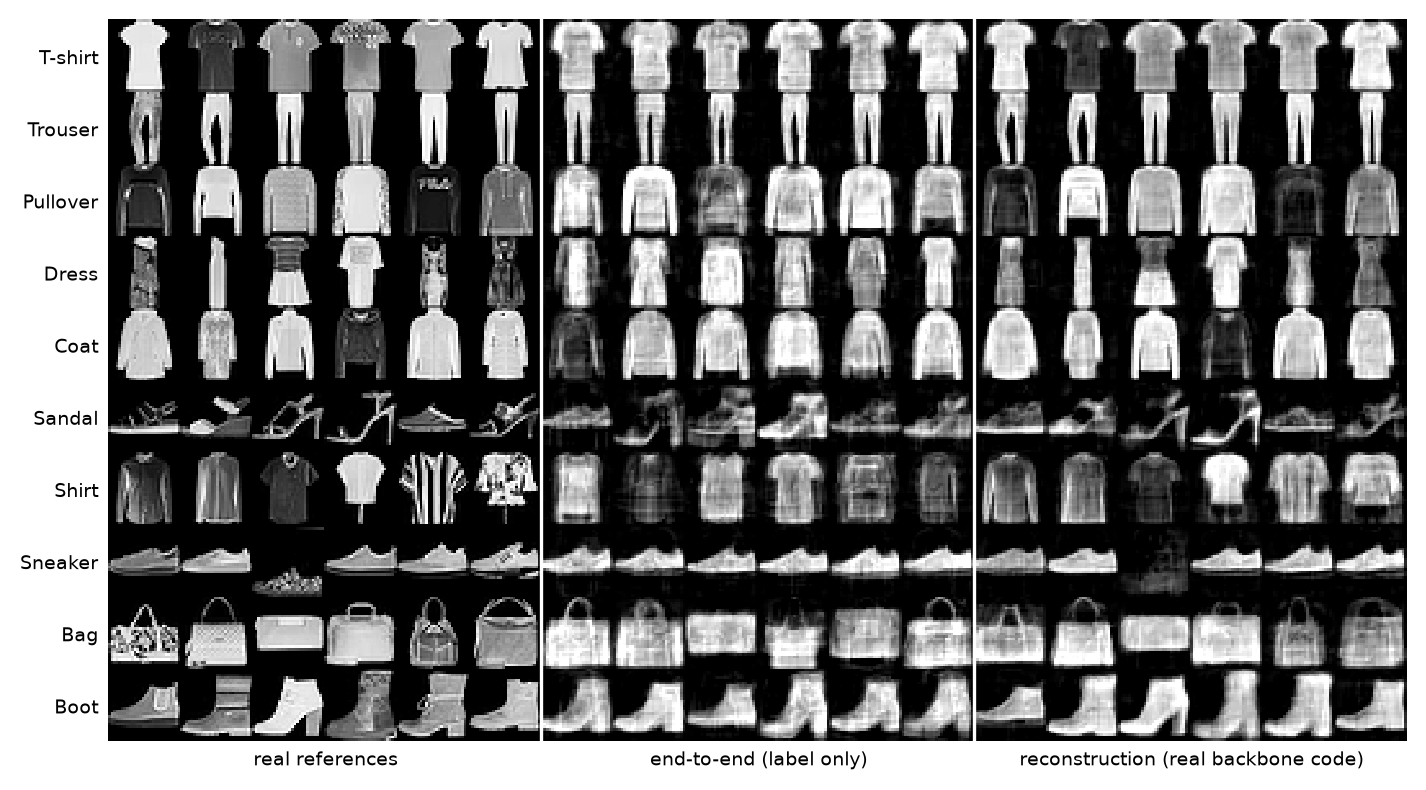
\includegraphics[width=\linewidth]{figures/fig-samples.png}
\captionof{figure}{Existing grayscale results: real images (left), generated from labels (center), and outputs supplied with real backbone codes (right). The first six samples per class from reporting seed 960 are shown without sample selection. These use the classifier-optimal noise setting, not the FID-optimal setting in the table.}
\end{center}
\vspace{-3pt}
The grayscale model's class agreement is about 90\%, similar to the real-image reference, but its tone variation is lower and its contrast is higher. A classifier can reward prototypes; this score does not establish equal image quality. The smaller one-level model illustrates a quality--energy tradeoff within the same architecture.

These are validation results: 68,000 images were used for fitting, and the remaining 2,000 informed model selection. The DTM uses the canonical 60,000-image training split. Binary training removes the richer grayscale training signal, but does not remove that split difference. FID also depends strongly on preprocessing, and does not by itself establish diversity or generalization.

\newpage
\section{Why the energy estimate is lower}
The principal comparison is with the DTM's proposed thermodynamic hardware. The DTM divides generation into denoising stages, each sampled through repeated local updates. Its eight-step configuration uses about ten million random conditional updates per image. CHILL ZEN uses 3,616 hot lane reads for generation. Including cold repair and the proposed decoder, its accounting covers 10,064 lane reads and about 1.78 million address assertions.

These operations are not equivalent. A CHILL ZEN lane read combines many stored weights, and its comparator is estimated to cost more than the DTM's random-number source per draw. Fewer draws alone therefore cannot establish an energy ratio. The paper separately counts address delivery, analog reads, and readout to estimate energy per completed image.

\subsection{The dominant cost is moving addresses}
At the nominal CHILL ZEN operating point, sending selection signals to the arrays accounts for about 91\% of energy. Readout contributes 8\%, and the analog divider reads about 1\%. The estimate includes a comparator and buffer for each lane read and a proposed lane decoder. The largest opportunity for further savings in this model is the selection circuitry and wiring.

\begin{center}
\small
\begin{tabularx}{\linewidth}{@{}>{\raggedright\arraybackslash}Xr>{\raggedright\arraybackslash}X@{}}
\toprule
Energy scenario & nJ/image & Interpretation \\
\midrule
Nominal CHILL ZEN & 2.0 & About one eighth of the DTM estimate \\
Selector-column design & 1.6 & Removes the nominal array's unwanted current paths \\
Pessimistic CHILL ZEN corner & 8.1 & About half of the DTM estimate \\
Published eight-step DTM & 15.7 & Reference from the DTM paper's figure \\
\bottomrule
\end{tabularx}
\end{center}

The nominal array allows current through unselected memory elements, whereas the quality emulator reads only selected elements. Its 2.0 nJ estimate is therefore not, by itself, a complete hardware realization of the demonstrated computation. The paper identifies a selector-column geometry that provides isolated reads at a modeled 1.6 nJ. This preserves the energy case at the array level, subject to the same unverified readout and decoder assumptions.

These scenarios are design calculations, not confidence intervals or bounds on all implementation costs. They exclude weight programming, host communication, and die area. In particular, in-memory decoder precision has not been demonstrated. The paper estimates that a digital decoder could add 1.8--8.9 nJ per image, materially reducing the advantage. Using the DTM paper's textual energy estimate instead of its figure changes the nominal ratio from 7.9 to 6.4.

\subsection{Latency is promising but conditional}
If a complete CHILL ZEN step fits a 62.5 nanosecond readout window, generation plus lane decoding would take about 8 microseconds. The DTM's stated sampling timings imply about 400 microseconds of single-image latency. The CHILL ZEN window has not been demonstrated as a complete instruction cycle, and a pipelined DTM could deliver images more frequently than its latency suggests. Neither figure establishes measured system throughput.

\newpage
\section{What remains between the model and a machine}
CHILL ZEN demonstrates generative computation organized around memory lanes. The existing study identifies three areas that determine whether its modeled advantages can translate into a working machine.

\subsection{Readout is the central unresolved component}
The comparator must combine adjustable noise, low static offset, suitable bandwidth, and low energy. At a 10 millivolt read voltage, the target offset is below about 1 millivolt at every operating bias. Noise must span the levels required for hot generation and cold repair. No designed circuit has demonstrated these requirements together. Switching inside the comparator can also disturb the small voltage it is measuring, an effect called kickback that is absent from the emulator.

Existing grayscale controls found no detectable change in aggregate image metrics when ideal cold reads were replaced by the modeled physical noise floor, despite changes in individual decisions. This supports some tolerance to cold-read noise. The headline FID comparison was not repeated with that floor, and the control does not establish circuit feasibility.

\subsection{Memory integration and decoding need validation}
The proposed selector-column array addresses unwanted current paths, but a lane-scale system has not been fabricated. The banks require roughly 57 million memristors; device count makes integration, programming, and area consequential even with low modeled energy per image. Physical memristors exist, but the emulator's device constants still need measurement. The proposed linear lane decoder also needs a precision check: current quality results use floating-point decoding on the host.

\subsection{The demonstrated workload is deliberately small}
The results support this representation and generation procedure on Fashion-MNIST. They do not establish scaling to richer data, superiority of local learning over gradient training, or an end-to-end training-energy advantage. The remaining statistical work includes an untouched test split and a controlled comparison with matched data and scoring. The energy model concerns inference; it does not determine product cost or commercial viability.

\takeaway{The architectural result is a useful generative procedure with a short, fixed sampling schedule. The hardware opportunity depends on realizing the lane readout, isolated memory access, and decoder within the stated energy budget.}

{\small\raggedright
\textbf{Sources.} Condensed from M.\ Alexander Nugent, \emph{From one to zero: Comparator-Heated In-memory Lane Learning with Zero-Ended Noise} (\texttt{main.tex}). The full paper supplies methods, controls, and references; \texttt{NUMBERS.md} maps results to evidence. Companion repository prepared for release: \url{https://github.com/knowm/CHILL-ZEN}.

\textbf{Comparison reference.} A.\ Jelin\v{c}i\v{c} et al., \emph{An efficient probabilistic hardware architecture for diffusion-like models}, arXiv:2510.23972v2 (2025). Scoring implementation: \url{https://github.com/pschilliOrange/dtm-replication}, commit \texttt{7c22d19}.

\textbf{Disclosure.} The author is part of Knowm Inc., which has sold memristors and plans products or intellectual property based on these technologies. The full paper details related patents and competing interests.
\par}
\end{document}
